% !TEX root = ../agglo_clust_review.tex

\section{Generalized framework for agglomerative clustering of signed graphs} \label{sec:general_framework}
In this section, we first define notation and then introduce one of our main contributions: a signed graph partitioning algorithm (Sec. \ref{sec:algorithm}) that can be seen as a generalization of several existing and new clustering algorithms (Sec. \ref{sec:alg_update_rules}).
 % introduces the proposed generalized framework: 
%that represents a simple \UPDATE{generalized} formalization of many agglomerative graph clustering algorithms. \UPDATE{It can be used to describe both unsigned clustering algorithms ingesting positive node similarities and signed clustering algorithms using attractive and repulsive cues.}\\
% we  in Sec.~\ref{sec:notation}, introduce Algorithm \ref{main_alg} in  and finally show how it can be seen as a generalization of existing and new graph clustering algorithms in .

\subsection{Notation and graph formalism} \label{sec:notation}

We consider an undirected simple edge-weighted graph $\mathcal{G}(V,E,w^+, w^-)$ with both attractive and repulsive edge attributes. In computer vision applications, the nodes can represent either pixels, superpixels or voxels. We call the set $\Pi$ a \emph{clustering} or \emph{partitioning} with $K$ clusters if $V = \cup_{S\in\Pi} S $, $\,S \cap S' = \emptyset$ for different clusters $S, S'\in \Pi$ and every cluster $S \in \Pi$ induces a connected subgraph of $\mathcal{G}$. We also denote as $S_u$ the cluster associated with node $u$.
% \begin{equation}
% S_u \equiv S \in \Pi \,\, \text{s.t.} \,\, u \in S
% \end{equation}
% In this work, we consider the problem of clustering a weighted graph $\mathcal{G}(V,E,w^+, w^-)$ with both attractive and repulsive edge attributes. 
The weight function $w^+: E \rightarrow \mathbb{R}^+$ associates to every edge a positive scalar attribute $w_e^+\in \mathbb{R}^+$ representing a merge affinity or a similarity measure: the higher this number, the higher the inclination of the two incident vertices to be assigned to the same cluster\footnote{Note that other formalisms for positively weighted graphs associate distances to the edges, thus, the \emph{lower} the edge weight, the higher the attraction between the two linked nodes, contrary to our definition of $w^+$.}. On the other hand, $w^-: E \rightarrow \mathbb{R}^+$ associates to each edge a split tendency $w_e^- \in \mathbb{R}^+$: the higher this weight, the more the incident vertices would like to be in different clusters. 
Graphs of the type $\mathcal{G}(V,E,w^+, w^-)$ are also often defined as \emph{signed graphs} $\mathcal{G}(V,E,\cost)$, featuring positive and negative edge weights $\cost_e\in \mathbb{R}$. Following the theoretical considerations in \cite{lange2018partial}, we define these signed weights as ${\cost_e = w_e^+ - w_e^-}$. Some approaches directly compute $\cost_e$, whereas others compute $w_e^+$ and $w_e^-$ separately.
In this formalism, graphs with purely attractive interactions are a special case of $\mathcal{G}(V,E,\cost)$ with $\cost_e \geq 0, \, \forall e \in E$.

\textbf{Inter-cluster interaction } We call two clusters $S_u,S_v$ \emph{adjacent} if there exists at least one edge ${e_{ts}\in E}$ connecting a node $t\in S_u$ to a node $s\in S_v$. In hierarchical agglomerative clustering, the interaction $\interact(S_u,S_v)$ between the two clusters is usually defined as a function $\interact{}:\Pi \times \Pi \rightarrow \mathbb{R}$, named \emph{linkage criterion}, depending on the weights of \emph{all} edges connecting clusters $S_u$ and $S_v$, i.e. $(S_u \times S_v) \cap E$. 
All the linkage criteria tested in this article are listed and defined in Table \ref{tab:linkage-criteria}.
% For example, for a \emph{maximum} linkage criterion statistic (single-linkage), the inter-cluster interaction is given by:
% \begin{equation}\label{eq:max_linkage}
% \interact_{S_1,S_2} = \, \max_{e\in U(S_u,S_v)} \cost(e), \qquad \text{where}\quad E_{12} = \{ e_{uv} \in E | u \in S_1, \, v \in S_2 \}.
% \end{equation}
% Other common choices are \emph{minimum} (complete linkage) or \emph{average} (average linkage). %and \emph{sum}.

\begin{figure}
\centering
        \begin{subfigure}[t]{0.46 \textwidth}
        \centering
        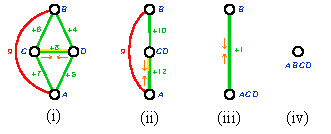
\includegraphics[width=\textwidth]{./figs/example_no_constr.pdf}
        \caption{No constraints}\label{subfig:no_constraints}
    \end{subfigure} \hfill
    \begin{subfigure}[t]{0.46 \textwidth}
        \centering
        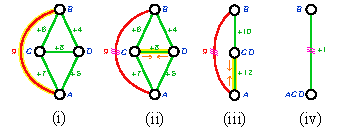
\includegraphics[width=\textwidth]{./figs/example_with_constr.pdf}
        \caption{With cannot-link constraints}\label{subfig:with_constraints}
    \end{subfigure}
\caption{Some iterations of the generalized algorithm (using \emph{Sum} linkage criteria) with and without adding cannot-link constraints. The graph has both attractive (green) and repulsive (red) edges and cannot-link constraints are shown with triple violet bars on the edges. We note that when constraints are enforced, the final clustering is given by two clusters instead of only one.}
\label{fig:algorithm_with_without_CLC}
\end{figure}
\begin{algorithm}[t]
  \caption{\algname{}: Generalized Algorithm for Agglomerative Signed Graph Partitioning}
   \hspace*{\algorithmicindent} \textbf{Input:} Graph $\mathcal{G}(V,E,w^+,w^-)$; linkage criterion $\interact{}$; boolean {\color{blue}\texttt{addCannotLinkConstraints}}  \\
  \hspace*{\algorithmicindent} \textbf{Output:} Final clustering $\Pi$\\
  \hspace*{\algorithmicindent} 
  \begin{algorithmic}[1]
      \State Initialize clustering $\Pi=\{\{v_1\}, \ldots, \{v_N\}\}$ with each node in its own cluster
      \State Initial interactions between nodes given by $\cost_e = w^+_e - w^-_e$
      % \State Initialize \texttt{canBeMerged}$[e] \gets$ \texttt{True} $\,\,\, \forall e\in E$
      % \State Sort edges in priority queue (PQ) in descending order of absolute weight $|\cost_e|=|w^+_e - w^-_e|$ 
      % \State
      \Repeat
        \State Select pair of clusters $S_u,S_v\in\Pi$ with highest absolute interaction $|\interact{}(S_u,S_v)|$
        % \State
        \If{\big[{\color{ForestGreen}\textbf{$\interact{}(S_u,S_v) > 0$}}\big] \textbf{and} \big[$S_u,S_v$ are \textbf{not} constrained\big]}
          \State Merge cluster $S_u$ with $S_v$: update interactions and cannot-link constraints with all their neighbors
        % \State
        \ElsIf{\big[{\color{red}\textbf{$\interact{}(S_u,S_v) \leq 0$}}\big] \textbf{and} {\color{blue}\texttt{addCannotLinkConstraints}}}
          \State Add CannotLink Constraint between clusters $S_u$ and $S_v$
        \EndIf
      \Until{\big[all interactions between clusters are repulsive\big] \textbf{or} \big[all adjacent clusters have cannot-link constraints\big]}
        % \If{({\color{ForestGreen}\textbf{$\interact{}(S_u,S_v) > 0$}}) \textbf{and} \texttt{canBeMerged}$[e_{uv}]$}
        %   \State Contract $e_{uv}$ in $\tilde{\mathcal{G}}_\Pi$ and merge the two clusters $S_u,S_v \in \Pi$
        %   \For{every new pair of double edges $(e_1,e_2)$ in $\tilde{\mathcal{G}}_\Pi$}
        %     % \State Get costs $\cost_1, \cost_2$ of $e_1,e_2$
        %     \State Delete $e_2$ from $\tilde{\mathcal{G}}_\Pi$ and update priority of $e_1$ with rule $f(\tilde{\cost}_{e_1},\tilde{\cost}_{e_2})$ defined in Tab. \ref{tab:linkage-criteria} 
        %   \EndFor
        % \EndIf
        % \If{({\color{red}\textbf{$\tilde{\cost} \leq 0$}}) \textbf{and} {\color{blue}\texttt{addCannotLink}}}
        %   \State \texttt{canBeMerged}$[e_{uv}] \gets$ \texttt{False}
        % \EndIf
      
      % \State
      \State
      \Return $\Pi$
  \end{algorithmic}
  \label{main_alg}
\end{algorithm}

\subsection{\algname{}: Generalized algorithm for agglomerative signed graph partitioning} \label{sec:algorithm} 

In Algorithm \ref{main_alg}, we provide a simplified pseudo-code for the proposed \algname{} algorithm that is based on a bottom-up approach starting with each node assigned to its own cluster and iteratively merging pairs of adjacent clusters. The algorithm has two variants, depending on the boolean value of the input option \texttt{addCannotLinkConstraints}. The first one, with \texttt{addCannotLinkConstraints=False}, starts by merging clusters with the strongest attractive interaction and it stops when the remaining clusters share only mutual repulsive interactions (see iterations on toy graphs in block 3 of Fig. \hyperref[fig:intro_figure]{\ref*{fig:intro_figure}}). After each merging iteration, the interaction between the merged cluster and its neighbors is updated according to one of the linkage criteria $\interact(S_u, S_v)$ listed in Table \ref{tab:linkage-criteria}.

In the second variant, when \texttt{addCannotLinkConstraints=True}, Algorithm \ref{main_alg} also introduces \emph{cannot-link constraints}, which represent mutual exclusion relationships between pairs of nodes that cannot be associated with the same cluster in the final clustering. This variant 
selects the pair of clusters with the highest absolute interaction $|\interact(S_u, S_v)|$, so that the most attractive and the most repulsive pairs are analyzed first (see example in Fig. \ref{subfig:with_constraints}). If the interaction is repulsive, then the two clusters are constrained. If it is attractive, then they are merged, provided that they were not already previously constrained. 
The algorithm stops when all the remaining clusters are constrained.
% The algorithm that we will present in the next section iteratively performs a sequence of so-called \emph{edge contractions} on the original graph $\mathcal{G}(V,E,w^+, w^-)$.
% The graph clustering algorithm we will present in Sec. \ref{sec:algorithm} is a bottom-up approach starting with each node assigned to its own cluster and iteratively merging clusters. During the agglomeration, the current clustering $\Pi$ is represented by a \emph{contracted graph} $\mathcal{G'}(\mathcal{G}, \Pi)$, such that each of its nodes represents a cluster $S \in \Pi$ and \emph{adjacent} clusters are linked by an edge. 
% For the linkage criteria tested in this work, when two clusters $S_u$ and $S_v$ are merged, the interactions between the new cluster $S_u \cup S_v$ and each of its neighbors depend only on the previous interactions involving $S_u$ and $S_v$. Thus, we can easily recompute these interactions by using a simple \emph{update rule} $f$ that does not involve any loop over the edges of the original graph $\mathcal{G}$. As an example, given the single-linkage criterion defined in Eq. \ref{eq:max_linkage}, the interaction between $S_u \cup S_v$ and one of its neighbors $S_t$ is simply given by:
% \begin{equation}
%   \interact_{S_u \cup S_v,S_t} = f( \interact_{S_u,S_t}, \interact_{S_v,S_t}) = f(\tilde{\cost}(e_{ut}), \tilde{\cost}(e_{vt})) = \max \{ \tilde{\cost}(e_{ut}), \tilde{\cost}(e_{vt}) \}
% \end{equation}
% All the update rules tested in this article are listed in Table \ref{tab:linkage-criteria}.

In Appendix \ref{sec:detailed_impl}, we comment on the algorithm computational complexity $\mathcal{O}(N^2 \log N)$ and present our efficient implementation given by the edge contraction Algorithm \ref{detailed_alg} using a priority queue.

% \UPDATE{\textbf{The proposed edge contraction algorithm } Algorithm \ref{main_alg} then proceeds as follows, similarly to the one presented in \cite{levinkov2017comparative}. It starts with each node assigned to its own cluster and sorts all edges $e\in E$ in a priority queue (PQ) by their absolute weight $|\cost_e|=|w_e^+ - w_e^-|$ in descending order, so that the most attractive and the most repulsive interactions are processed first. It then iteratively pops one edge $e_{uv}$ from PQ and, depending on the priority $\tilde{\cost}$, does the following: in case of attractive interaction $\tilde{\cost}>0$, provided that $e_{uv}$ was not flagged as a cannot-link constraint, then merge the connected clusters, perform an edge contraction of $e_{uv}$ in $\tilde{\mathcal{G}}_\Pi$ and update the priorities of new double edges as explained in Fig. \ref{fig:edge_contraction_and_contr_graph}. 
% % For every new pair of double edges in $\tilde{\mathcal{G}}_\Pi$, update their priorities according to one of the update rules listed in Table \ref{tab:linkage-criteria} together with their cannot-link relationships. 
% If, on the other hand, the interaction is repulsive ($\tilde{\cost}\leq 0$) and the option \texttt{addCannotLink} of Alg. \ref{main_alg} is \texttt{True}, then the edge $e_{uv}$ is flagged as cannot-link constraint.
% In the Supplementary material we comment on the algorithm computational complexity (Sec. \ref{sec:complexity}).}

 %\TODO{use def of merging process of contracted graph to define merging tree?}.

% \item Comment about must-not-link relations: they give high priority to the most confident repulsive edges {}


% Given a clustering $\Pi$ and a graph $\mathcal{G}(V,E,W)$, the interaction between two clusters $S_1, S_2 \in \Pi$ is usually defined in terms of a \emph{linkage criterion}, i.e. a function of all the edge weights connecting the two clusters:
% \begin{equation} 
% \begin{gathered}
% \mathcal{L}(S_1,S_2) = \mathcal{L}(\mathcal{W})\quad \\
%    \text{where} \quad \mathcal{W} = \{ W(e_{uv})| u\in S_1, v\in S_2 \}.
% \end{gathered}
% \end{equation}


\begin{table*}
    \centering
    \scriptsize
    \begin{subtable}[t!]{\textwidth}\centering
        \begin{tabular}{c r  l | c | c  c}
            % \toprule\toprule
            \multicolumn{3}{c|}{\multirow{2}{*}[-0.5em]{\thead{\textbf{Linkage criteria} $\,\,\interact(S_u ,S_v)$}}}  & \multirow{2}{*}[-0.5em]{\thead{\textbf{Unsigned Graphs}}} & \multicolumn{2}{c}{\thead{\textbf{Signed Graphs}}}  \\        
            % \cmidrule(l{.15em}){4-5}
            % \cline{4-5}
            % \multicolumn{2}{c||}{} &  &  \multicolumn{2}{c}{\thead{Add Cannot-Link Constraints:}} \\        
            \multicolumn{3}{c|}{} &  &  \multicolumn{1}{c}{\thead{No Constraints}} & \thead{With Constraints} \\        
      
            \midrule
            % \cmidrule[0.3em]{2-6}
            % \morecmidrules \cmidrule[0.15em]{2-6}
            % \midrule \midrule
            % \multirow{5}{*}[-0.5em]{\begin{turn}{90}\thead{\textbf{Linkage criteria} $\,\,\interact(S_u ,S_v)$}\end{turn}} 
             & Sum: & $\displaystyle \sum_{e\in E_{uv}} \cost_e$ & \thead{Sum Linkage\\Hier. Aggl. Clust.} & \thead{GAEC \cite{keuper2015efficient}} & \thead{Greedy Fixation \cite{levinkov2017comparative}} \\ 
            % \cmidrule[0.07em]{2-6}
            
             &\makecell[r]{Absolute Max:} & 
            $\displaystyle \cost_e$ with $\displaystyle e = \argmax_{t\in E_{uv}} |\cost_t|$
               & \thead{Single Linkage\\Hier. Aggl. Clust.} & \thead{Mutex Watershed \cite{wolf2018mutex}} & \thead{Mutex Watershed \cite{wolf2018mutex}} \\
              % \cmidrule[0.07em]{2-6}
             & \makecell[r]{Average:} & $\displaystyle \sum_{e\in E_{uv}} \cost_e \bigg/ \big|E_{uv}\big|  $ & \thead{ Average Linkage\\ Hier. Aggl. Clust.} & \thead{\textbf{NEW}} & \thead{\textbf{NEW}}\\ 
            % \cmidrule[0.07em]{2-6}
           % \midrule

            & Max: & $\displaystyle \max_{e\in E_{uv}} \cost_e$ & \thead{Single Linkage\\Hier. Aggl. Clust.} & \thead{\textbf{NEW}} & \thead{\textbf{NEW}}\\ 
            % \cmidrule[0.07em]{2-6}

            & Min:& $\displaystyle \min_{e\in E_{uv}} \cost_e$ & \thead{Complete Linkage\\ Hier. Aggl. Clust.}  & \thead{\textbf{NEW}} & \thead{\textbf{NEW}}



            
        \end{tabular}
        % \caption{Linkage criteria}
    \end{subtable} 
    \caption{The table lists the existing clustering algorithms that can be reformulated as special cases of the proposed generalized algorithm \algname{}, given a linkage criteria, a type of graph (signed or unsigned) and the optional use of cannot-link constraints. The set $E_{uv}$ is defined as the set of all edges connecting cluster $S_u$ to cluster $S_v$, i.e. $E_{uv}=(S_u \times S_v) \cap E$.}
    \label{tab:linkage-criteria}
\end{table*}
\begin{figure}
\centering
% 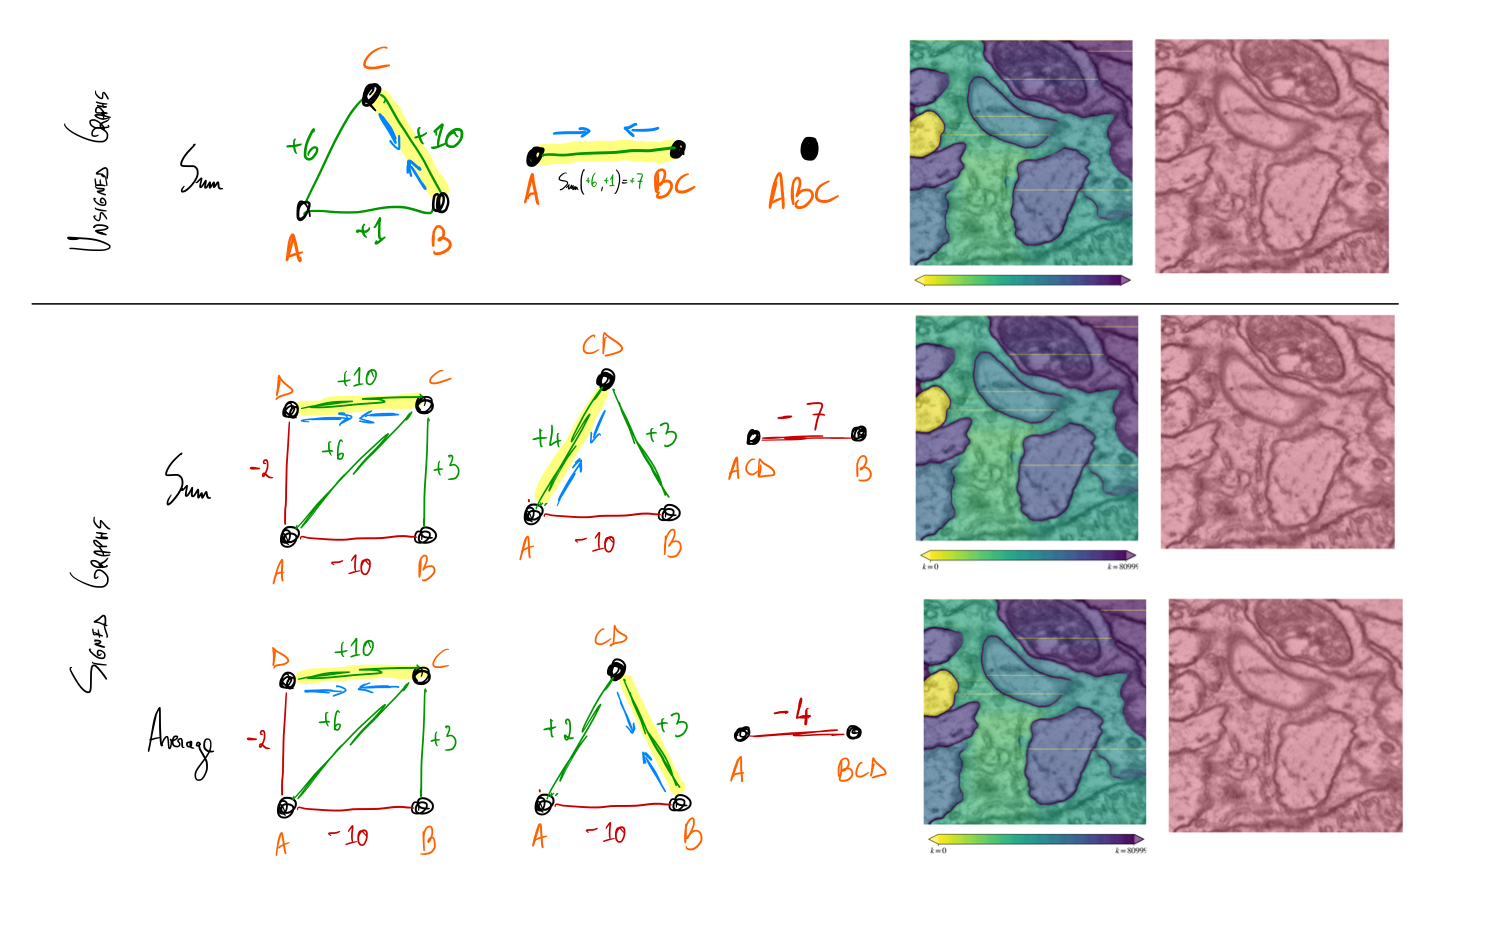
\includegraphics[width=0.5\textwidth,trim=0.4in 1.2in 0.in 0.05in,clip]{./figs/intro_image.jpg} % left bottom right top
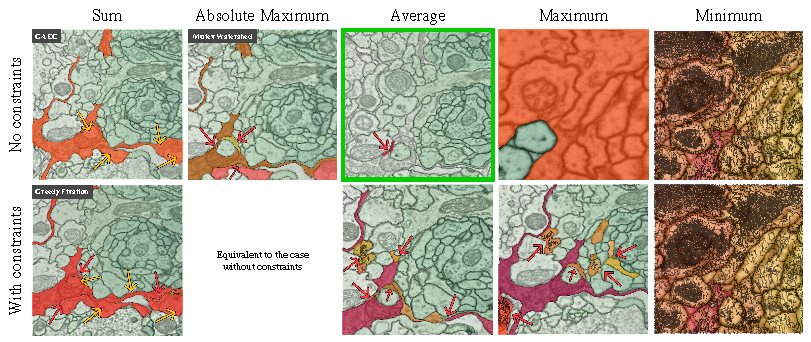
\includegraphics[width=0.9\textwidth]{./figs/comparison_new.pdf} % left bottom right top
\caption{Failure cases of \algname{} with different linkage criteria highlighted on some difficult parts of the CREMI Challenge data. The main \emph{wrongly} segmented regions are highlighted in different warm colors. Note that the data is 3D, hence the same color could be assigned to parts of segments that appear disconnected in 2D.  Red arrows point to wrongly split regions. Yellow arrows point out merge errors. The \emph{Average} linkage without cannot-link constraints returned the best segmentation.
% Only the involved segments are colored.
 % main ideas and contributions
\label{fig:cremi_comparison}}
\end{figure}



% \begin{table*}
%     \centering
%     \scriptsize
%     \begin{subtable}[t!]{\textwidth}\centering
%         \begin{tabular}{r  l || c | c | c}
%             % \toprule\toprule
%             \multicolumn{2}{c||}{}  &   & \multicolumn{2}{c}{\textbf{Signed graphs}}  \\        
%             % \cmidrule(l{.15em}){4-5}
%             % \cline{4-5}
%             \multicolumn{2}{c||}{} & \textbf{Unsigned graphs} &  \multicolumn{2}{c}{\thead{Add Cannot-Link Constraints:}} \\        
%              &  &  &  \thead{\textsc{No}} & \thead{\textsc{Yes}} \\        
%             % \cmidrule[0.3em]{3-5}
%             % \midrule[0.15em]
%             \midrule\midrule
%             Sum: & \thead[l]{$f(\tilde{\cost}_1,\tilde{\cost}_2) = \tilde{\cost}_1+\tilde{\cost}_2$} & \thead{Sum Linkage\\Hier. Aggl. Clust.} & \thead{Greedy Additive \\ Edge Contraction \cite{keuper2015efficient}} & \thead{Greedy Fixation\\\cite{levinkov2017comparative}} \\ \midrule
            
%             \makecell[r]{Absolute \\Max:} & \thead[l]{
%             $
%             f(\tilde{\cost}_1,\tilde{\cost}_2) = \begin{cases} 
%             \tilde{\cost}_1 & \text{if}\,\, |\tilde{\cost}_1|>|\tilde{\cost}_2|\\
%             \tilde{\cost}_2 & \text{otherwise}
%              \end{cases} 
%             $}
%                & \thead{Single Linkage\\Hier. Aggl. Clust. \cite{lance1967general}} & \thead{Mutex Watershed \\\cite{wolf2018mutex}} & \thead{Mutex Watershed\\\cite{wolf2018mutex}} \\ \midrule
%             \makecell[r]{Mean:} & \thead[l]{$f(\tilde{\cost}_1,\tilde{\cost}_2) = \mathrm{weightAvg}\{ \tilde{\cost}_1, \tilde{\cost}_2 \} $}                                 & \thead{ Average Linkage\\ Hier. Aggl. Clust. \cite{lance1967general}} & \thead{Average Linkage\\Signed Aggl. Clust. (\textbf{NEW})} & \thead{\textbf{NEW}}\\ \midrule

%             Max: & \thead[l]{$f(\tilde{\cost}_1,\tilde{\cost}_2) = \max \{ \tilde{\cost}_1, \tilde{\cost}_2 \}  $}                                 & \thead{Single Linkage\\Hier. Aggl. Clust. \cite{lance1967general}} & \thead{Single Linkage \\Signed Aggl. Clust. (\textbf{NEW})} & \thead{\textbf{NEW}}\\ \midrule

%             Min:& \thead[l]{$f(\tilde{\cost}_1,\tilde{\cost}_2) = \min \{ \tilde{\cost}_1, \tilde{\cost}_2 \}  $}                                 & \thead{Complete Linkage\\ Hier. Aggl. Clust. \cite{lance1967general}}  & \thead{Complete Linkage \\Signed Aggl. Clust. (\textbf{NEW})} & \thead{\textbf{NEW}}



            
%         \end{tabular}
%         % \caption{Linkage criteria}
%     \end{subtable} 
%     \caption{{\small The table lists the tested update rules $f$. Existing and new algorithms are given by a specific choice of update rule, type of graph (signed or unsigned) and optional use of cannot-link constraints.}}
%     \label{tab:linkage-criteria}
% \end{table*}



\subsection{\algname{} with different linkage criteria: new and existing algorithms} \label{sec:alg_update_rules}
%In this section, we show how the choice of different update rules for the presented generalized algorithm \algname{} leads to existing and new algorithms (see Table \ref{tab:linkage-criteria}).

In the special case of an unsigned graph with only positive interactions, i.e. $w_e^-=0$ and $\cost_e \geq 0$ $\forall e\in E$, %$\mathcal{G}(V,E,W:E\rightarrow \mathbb{R}^+)$ 
 the algorithm performs a standard agglomerative hierarchical clustering by returning only a single cluster and a hierarchy of clusters defined by the order in which the clusters are merged (see Table \ref{tab:linkage-criteria}, unsigned graphs).

Given a graph with both attractive and repulsive cues, an edge contraction algorithm with a sum update rule was already proposed in \cite{levinkov2017comparative,keuper2015efficient} (Table \ref{tab:linkage-criteria}, \emph{Sum} linkage). They present both a version with cannot-link constraints and one without, and then compare them with other greedy local-search algorithms solving the multicut optimization problem.
The Mutex Watershed \cite{wolf2018mutex} is another signed graph partitioning algorithm that introduces dynamical cannot-link constraints. In Appendix \ref{sec:appendix_abs_max} we prove that it can be seen as an efficient implementation of \algname{} with \emph{Absolute maximum} linkage (see def. in Table \ref{tab:linkage-criteria}) and observe that in this case \algname{} returns the same clustering with or without enforcing cannot-link constraints.
On the other hand, to our knowledge, \emph{Average}, \emph{Max} or \emph{Min} linkage criteria have never been used for signed graphs agglomerative algorithms or been combined with cannot-link constraints.

Apart from the linkage criteria defined in Table \ref{tab:linkage-criteria}, additional ones were proposed in the literature:
\cite{nunez2013machine} for example uses a learned approach where a random forest classifier updates the cluster interactions depending on predefined edge and node features; other approaches introduce a weight regularization depending on the size of the clusters \cite{felzenszwalb2004efficient,kardoostsolving}, whereas 
\cite{funke2018large} uses a \emph{quantile} linkage criteria by populating a histogram for each inter-cluster interaction. In our experiments, we decided to focus on the linkage criteria listed in Table \ref{tab:linkage-criteria}, since they represent the most common options.

